
\label{sec:prestazioni_ramjet}
\hspace{2cm}
\section{Prestazioni}


\begin{figure}[H]
    \centering


    %------------------------------------------------
    % CICLO TERMODINAMICO A SINISTRA
    %------------------------------------------------
    \begin{minipage}[c]{0.64\linewidth}
        \centering
        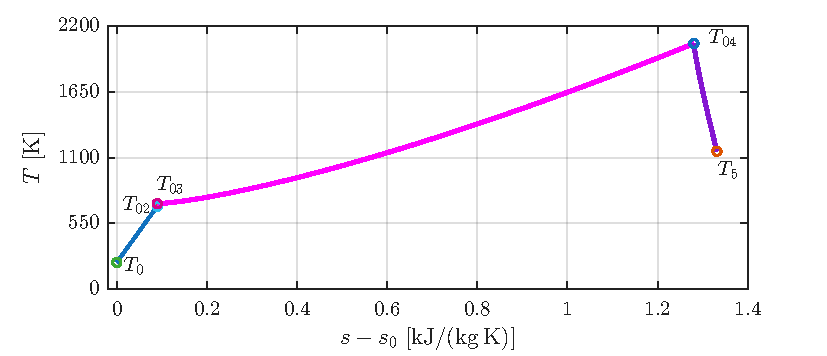
\includegraphics[width=\linewidth]
        {Graphics/ramjet/ciclo_termodinamico_ramjet.pdf}
    \end{minipage}
    \hfill
   %------------------------------------------------
% TABELLA PRESSIONI E TEMPERATURE TOTALI A DESTRA
%------------------------------------------------
\begin{minipage}[c]{0.33\linewidth}
    \centering
    \renewcommand{\arraystretch}{1}
    \fontsize{11pt}{11pt}\selectfont
    \caption{Pressioni e temperature nei punti del ciclo.}
    \begin{tabular}{ccc}
        \toprule
        \textbf{Punto} &
        \textbf{$P$ [kPa]} &
        \textbf{$T$ [K]} \\
        \midrule
        $0$ & 2.55 & 221 \\
        $02$ & 142  & 765 \\
        $03$ & 142  & 765 \\
        $04$ & 137  & 2100 \\
        $5$ & 10.2  & 1150 \\
        \bottomrule
    \end{tabular}
\end{minipage}

\caption{Ciclo termodinamico del ramjet e principali grandezze totali
nelle stazioni del motore.}
\label{fig:prestazioni_ciclo_ramjet}
\end{figure}


\begin{table}[H]
\centering
\renewcommand{\arraystretch}{1}
\fontsize{11pt}{11pt}\selectfont
\caption{Prestazioni principali del ramjet, calcolate secondo la procedura riportata in Appendice~\ref{appC:prestazioni}.}
\label{tab:prestazioni_ramjet}
\begin{tabular}{lrl}
\toprule
\textbf{Parametro} & \textbf{Valore} & \textbf{Unità} \\
\midrule
Spinta                    & 65.0    & kN \\
Spinta specifica         & 643 & m/s \\
TSFC                      & 0.231 & kg/(N$\cdot$h) \\
Rendimento propulsivo     & 81.7  & \% \\
Rendimento termodinamico  & 45.7  & \% \\
Rendimento globale        & 37.4  & \% \\
\bottomrule
\end{tabular}
\end{table}
I principali risultati prestazionali ottenuti nel punto di progetto del ramjet ($M_0=3.5$, $h=25000$ m) sono riportati in Tabella~\ref{tab:prestazioni_ramjet}. Il TSFC ottenuto, pari a $0.231\ \mathrm{kg/(N\,h)}$, risulta inferiore
al limite di $0.278\ \mathrm{kg/(N\,h)}$ imposto dal vincolo di missione
(Appendice~A.3). Il rendimento propulsivo raggiunge l'$81.7\%$: il valore
elevato è associato al ridotto scarto tra la velocità di efflusso e quella
di volo, condizione favorevole alla conversione dell'energia cinetica del
getto in spinta utile. Il rendimento termodinamico risulta pari al
$45.7\%$, mentre dalla combinazione dei due contributi si ottiene un
rendimento globale del $37.4\%$.

\begin{table}[H]
\centering
\renewcommand{\arraystretch}{1}
\fontsize{11pt}{11pt}\selectfont
\caption{Portate massiche del ramjet nel punto di progetto.}
\label{tab:mass_ramjet}
\small
\begin{tabular}{lrl}
\toprule
\textbf{Parametro} & \textbf{Valore} & \textbf{Unità} \\
\midrule
$\dot{m}_{\text{aria}}$         & 101 & kg/s \\
$\dot{m}_{\text{combustibile}}$ & 4.18   & kg/s \\
$\dot{m}_{\text{totale (gas)}}$ & 105 & kg/s \\
\bottomrule
\end{tabular}
\end{table}

Nel punto di progetto il ramjet elabora una portata d'aria di
$101\ \mathrm{kg/s}$, alla quale si aggiungono $4.18\ \mathrm{kg/s}$ di
combustibile, ottenendo una portata complessiva dei gas pari a
$105\ \mathrm{kg/s}$. La maggiore portata d'aria rispetto al turbogetto
è associata alle differenti condizioni operative e, in particolare, alla
maggiore spinta richiesta, pari a $65\ \mathrm{kN}$.

Nel modello del ramjet non sono previsti spillamenti di portata per il
raffreddamento delle turbomacchine, assenti in questa configurazione.
Ciò consente inoltre di adottare una temperatura totale a valle della
combustione pari a $T_{04}=2100\ \mathrm{K}$, superiore alla temperatura
massima imposta nel dimensionamento del turbogetto dalla presenza della
turbina.

Il vincolo geometrico sul diametro di efflusso ($D_{eflusso}<1.6$ m, Tabella 1.4) risulta rispettato, con $D_E=1.57\ \mathrm{m}$: tale vincolo, introdotto proprio per evitare un'espansione completa fino alla pressione ambiente alla quota di crociera (che alle alte quote comporterebbe aree di efflusso eccessive), si riflette in un ugello volutamente sottoespanso, con pressione statica in uscita $P_E=10.2\ \mathrm{kPa}$ superiore alla pressione ambiente $P_0=2.5\ \mathrm{kPa}$ a $25000$ m. Questa scelta comporta una perdita di spinta rispetto all'espansione ottima, compensata dal contenimento dell'ingombro trasversale del propulsore, coerentemente con l'obiettivo di integrazione del ramjet nella configurazione a ciclo variabile con il turbogetto.